%!TEX root = modelguide.tex

% listings description environment
\let\olditem\item
\newcommand{\lstitem}[2][]{\olditem[{\protect\texttt{#1}}]\mbox{}\newline#2}
\newenvironment{lstdescription}{%
   \iflatexml
   \begin{description}
   \else
   \begin{description}[nolistsep]
   \fi
   \let\item\lstitem
}{\end{description}}

\newenvironment{tightemize}{%
   \iflatexml
   \begin{itemize}
   \else
   \begin{itemize}[nolistsep,noitemsep]
   \fi
}{\end{itemize}}


\chapter{DICOM Images}
\label{sec:dicom}

Some models are derived from image data, and it may be useful to show the model
and image in the same space.  For this purpose, a DICOM image widget has been designed,
capable of displaying 3D DICOM volumes as a set of three perpendicular planes.  An
example widget and its property panel is shown in Figure \ref{fig:dicom:heart}.

\begin{figure}[!ht]
   \begin{center}
      \setlengthLaTeXML{\imglength}{\textwidth}{0.8\textwidth}
      \includegraphics[width=\imglength]{images/dicom_heart}
      \caption{DICOM image of the heart, 
      downloaded from \url{http://www.osirix-viewer.com}. \label{fig:dicom:heart}}
   \end{center}
\end{figure}

The main classes related to the reading and displaying of DICOM images are:
\begin{lstdescription}
   \item[{\protect \javaclass[maspack.image.dicom]{DicomElement}}] Describes a single attribute in a DICOM file.
   \item[{\protect \javaclass[maspack.image.dicom]{DicomHeader}}] Contains all header attributes (all but the image data) extracted from a DICOM file.
   \item[{\protect \javaclass[maspack.image.dicom]{DicomPixelBuffer}}] Contains the \emph{decoded} image pixels for a single image frame.
   \item[{\protect \javaclass[maspack.image.dicom]{DicomSlice}}] Contains both the header and image information for a single 2D DICOM slice.
   \item[{\protect \javaclass[maspack.image.dicom]{DicomImage}}] Container for DICOM slices, creating a 3D volume (or 3D + time)
   \item[{\protect \javaclass[maspack.image.dicom]{DicomReader}}] Parses DICOM files and folders, appending information to a \javaclass[maspack.image.dicom]{DicomImage}. 
   \item[{\protect \javaclass[artisynth.core.renderables]{DicomViewer}}] Displays the \javaclass[maspack.image.dicom]{DicomImage} in the viewer.
\end{lstdescription}
If the purpose is simply to display a DICOM volume in the ArtiSynth viewer, then only the last three classes will be of interest.  Readers who simply want to display a DICOM image in their model can skip to Section \ref{sec:dicom:loading}.

\section{The DICOM file format}

For a complete description of the DICOM format, see the specification page at \url{http://medical.nema.org/standard.html}.  A brief
description is provided here.  Another excellent resource is the blog by Roni Zaharia: \url{http://dicomiseasy.blogspot.ca/}.

Each DICOM file contains a number of concatenated attributes (a.k.a.~elements), one of which defines the embedded binary image pixel data.  The other attributes act as meta-data, which can contain identity information of the subject, equipment settings when the image was acquired, spatial and temporal properties of the acquisition, voxel spacings, etc\ldots.  The image data typically represents one or more 2D images, concatenated, representing slices (or `frames') of a 3D volume whose locations are described by the meta-data.  This image data can be a set of raw pixel values, or can be encoded using almost any image-encoding scheme (e.g.~JPEG, TIFF, PNG).  For medical applications, the image data is typically either raw or compressed using a lossless encoding technique.  Complete DICOM acquisitions are typically separated into multiple files, each defining one or few frames.  The frames can then be assembled into 3D image `stacks' based on the meta-information, and converted into a form appropriate for display.

\begin{table}[ht]
   \centering
   \caption{A selection of Value Representations \label{tbl:dicom:vr}}
   \smallskip
   \begin{tabular}{|cl|}
      \hline
      VR & Description\\
      \hline
      CS & Code String \\ 
      DS & Decimal String \\ 
      DT & Date Time \\ 
      IS & Integer String \\ 
      OB & Other Byte String \\ 
      OF & Other Float String \\ 
      OW & Other Word String \\ 
      SH & Short String \\
      UI & Unique Identifier \\ 
      US & Unsigned Short \\ 
      OX & One of OB, OW, OF\\
      \hline
   \end{tabular}
\end{table}

Each DICOM attribute is composed of:
\begin{tightemize}
   \item a standardized unique integer \emph{tag} in the format (\texttt{XXXX},\texttt{XXXX}) that defines the \emph{group} and \emph{element} of the attribute
   \item a \emph{value representation} (VR) that describes the data type and format of the attribute's value (see Table \ref{tbl:dicom:vr})
   \item a \emph{value length} that defines the length in bytes of the attribute's value to follow
   \item a \emph{value field} that contains the attribute's value
\end{tightemize}
This layout is depicted in Figure \ref{fig:dicom:attribute}.  A list of important attributes are provided in Table \ref{tbl:dicom:attribute}.
\begin{figure}[ht]
   \centering
   \begin{tabular}{|c|c|c|c|}
      \hline
      Tag & VR & Value Length & \hspace*{8ex}Value Field\hspace*{8ex}\\
      \hline
   \end{tabular}%
   \iflatexml
   \else
   \vspace*{-0.75em}
   \fi
   \caption{DICOM attribute structure \label{fig:dicom:attribute}}
\end{figure}
\begin{table}[ht]
   \centering
   \caption{A selection of useful DICOM attributes \label{tbl:dicom:attribute}}
   \smallskip
   \begin{tabular}{|lcc@{, }c|}
      \hline
      Attribute name & VR & \multicolumn{2}{c|}{Tag}\\
      \hline
      Transfer syntax UID & UI & 0x0002 & 0x0010\\[0.5em]
      Slice thickness & DS & 0x0018 & 0x0050\\
      Spacing between slices & DS & 0x0018 & 0x0088\\[0.5em]
      Study ID & SH & 0x0020 & 0x0010\\
      Series number & IS & 0x0020 & 0x0011\\
      Aquisition number & IS & 0x0020 & 0x0012\\
      Image number & IS & 0x0020 & 0x0013\\
      Image position patient & DS & 0x0020 & 0x0032\\
      Image orientation patient & DS & 0x0020 & 0x0037\\
      Temporal position identifier & IS & 0x0020 & 0x0100\\
      Number of temporal positions & IS & 0x0020 & 0x0105\\
      Slice location & DS & 0x0020 & 0x1041\\[0.5em]
      Samples per pixel & US & 0x0028 & 0x0002\\
      Photometric interpretation & CS & 0x0028 & 0x0004\\
      Planar configuration (color) & US & 0x0028 & 0x0006\\
      Number of frames & IS & 0x0028 & 0x0008\\
      Rows & US & 0x0028 & 0x0010\\
      Columns & US & 0x0028 & 0x0011\\
      Pixel spacing & DS & 0x0028 & 0x0030\\
      Bits allocated & US & 0x0028 & 0x0100\\
      Bits stored & US & 0x0028 & 0x0101\\
      High bit & US & 0x0028 & 0x0102\\
      Pixel representation & US & 0x0028 & 0x0103\\[0.5em]
      Pixel data & OX & 0x7FE0 & 0x0010\\
      \hline
   \end{tabular}
\end{table}

\section{The DICOM classes}

Each \javaclass[maspack.image.dicom]{DicomElement} represents a single attribute contained in a DICOM file.
The \javaclass[maspack.image.dicom]{DicomHeader} contains the collection of \code{DicomElement}s defined in a file, 
apart from the pixel data.  The image pixels are decoded and stored in a \javaclass[maspack.image.dicom]{DicomPixelBuffer}.  
Each \javaclass[maspack.image.dicom]{DicomSlice} contains a \code{DicomHeader}, as well as
the decoded \code{DicomPixelBuffer} for a single slice (or `frame').  All slices are assembled into a single 
\javaclass[maspack.image.dicom]{DicomImage}, which can be used to extract 3D voxels and spatial locations from the set of slices.  
These five classes are described in further detail in the following sections.

\subsection{\texttt{DicomElement}}

The \javaclass[maspack.image.dicom]{DicomElement} class is a simple container for DICOM attribute information.  It has
three main properties:
\begin{tightemize}
\item an integer \emph{tag}
\item a \emph{value representation} (VR)
\item a value
\end{tightemize}
These properties can be obtained using the corresponding \code{get} function: \code{getTag()}, \code{getVR()}, \code{getValue()}.  The tag refers to the concatenated group/element tag. For example, the \emph{transfer syntax UID} which corresponds to group 0x0002 and element 0x0010 has a numeric tag of 0x00020010. The VR is represented by an enumerated type, \javaclass[maspack.image.dicom]{DicomElement\$VR}.  The `value' is the \emph{raw} value extracted from the DICOM file.  In most cases, this will be a \code{String}.  For raw numeric values (i.e.~stored in the DICOM file in binary form) such as the unsigned short (US), the `value' property is exactly the numeric value.

For VRs such as the integer string (IS) or decimal string (DS), the string will still need to be parsed in order to extract the appropriate sequence of numeric values.  There are static utility functions for handling this within \code{DicomElement}.  For a `best-guess' of the desired parsed value based on the VR, one can use the method \code{getParsedValue()}.  Often, however, the desired value is also context-dependent, so the user should know a priori what type of value(s) to expect.  Parsing can also be done automatically by querying for values directly through the \code{DicomHeader} object.  

\subsection{\texttt{DicomHeader}}

When a DICOM file is parsed, all meta-data (attributes apart from the actual pixel data) 
is assembled into a \javaclass[maspack.image.dicom]{DicomHeader} object.  This essentially acts
as a map that can be queried for attributes using one of the following methods:
\begin{lstlisting}[]
   DicomElement getElement(int tag);               // includes VR and data
   String getStringValue(int tag);                 // all non-numeric VRs
   String[] getMultiStringValue(int tag);          // UT, SH
   int getIntValue(int tag, int defaultValue);     // IS, DS, SL, UL, SS, US
   int[] getMultiIntValue(int tag);                // IS, DS, SL, UL, SS, US
   double getDecimalValue(int tag, double defaultValue);    // DS, FL, FD
   double[] getMultiDecimalValue(int tag);         // DS, FL, FD
   VectorNd getVectorValue(int tag);               // DS, IS, SL, UL, SS, US, FL, FD
   DicomDateTime getDateTime(int tag);             // DT, DA, TM
\end{lstlisting}
The first method returns the full element as described in the previous section.  
The remaining methods are used for convenience when the desired value type is known for the given tag.  
These methods automatically parse or convert the \code{DicomElement}'s value to the desired form.

If the tag does not exist in the header, then the \code{getIntValue(...)} and
\code{getDecimalValue(...)} will return the supplied \code{defaultValue}.  All other methods
will return \code{null}.

\subsection{\texttt{DicomPixelBuffer}}

The \javaclass[maspack.image.dicom]{DicomPixelBuffer} contains the decoded image information of an image slice.
There are three possible pixel types currently supported:
\begin{tightemize}
   \item byte grayscale values (\code{PixelType.BYTE})
   \item short grayscale values (\code{PixelType.SHORT})
   \item byte RGB values, with layout \code{RGBRGB...RGB} (\code{PixelType.BYTE\_RGB})
\end{tightemize}
The pixel buffer stores all pixels in one of these types.  The pixels can be queried for directly
using \code{getPixel(idx)} to get a single pixel, or \code{getBuffer()} to get the
entire pixel buffer.  Alternatively, a \javaclass[maspack.image.dicom]{DicomPixelInterpolator} object
can be passed in to convert between pixel types via one of the following methods:
\begin{lstlisting}[]
public int getPixelsByte (
   int x, int dx, int nx, byte[] pixels, int offset, DicomPixelInterpolator interp);

public int getPixelsShort (
   int x, int dx, int nx, short[] pixels, int offset, DicomPixelInterpolator interp);

public int getPixelsRGB (
   int x, int dx, int nx, byte[] pixels, int offset, DicomPixelInterpolator interp);

public int getPixels(
   int x, int dx, int nx, DicomPixelBuffer pixels, int offset, 
   DicomPixelInterpolator interp);
\end{lstlisting}
These methods populate an output array or buffer with converted pixel values, which can later
be passed to a renderer.  For further details on these methods, refer to the Javadoc documentation.

\subsection{\texttt{DicomSlice}}

A single DICOM file contains both header information, and one or more image `frames' (slices).  In
ArtiSynth, we separate each frame and attach them to the corresponding header information in
a \javaclass[maspack.image.dicom]{DicomSlice}.  Thus, each slice contains a single \code{DicomHeader} and 
\code{DicomPixelBuffer}.  These can be obtained using the methods: \code{getHeader()} and
\code{getPixelBuffer()}.  

For convenience, the \code{DicomSlice} also has all the same methods 
for extracting and converting between pixel types as the \code{DicomPixelBuffer}.

\subsection{\texttt{DicomImage}}

An complete DICOM acquisition typically consists of multiple slices forming a 3D image stack,
and potentially contains multiple 3D stacks to form a dynamic 3D+time image.  The collection
of \code{DicomSlice}s are thus assembled into a \javaclass[maspack.image.dicom]{DicomImage}, 
which keeps track of the spatial and temporal positions.

The \code{DicomImage} is the main object to query for pixels in 3D(+time).  To access pixels,
it has the following methods:
\begin{lstlisting}[]
public int getPixelsByte (
   int x, int y, int z, int dx, int dy, int dz, int nx, int ny, int nz, 
   int time, byte[] pixels, DicomPixelInterpolator interp);

public int getPixelsShort (
   int x, int y, int z, int dx, int dy, int dz, int nx, int ny, int nz, 
   int time, short[] pixels, DicomPixelInterpolator interp);

public int getPixelsRGB (
   int x, int y, int z, int dx, int dy, int dz, int nx, int ny, int nz, 
   int time, byte[] pixels, DicomPixelInterpolator interp);

public int getPixels (
   int x, int y, int z, int dx, int dy, int dz, int nx, int ny, int nz, 
   int time, DicomPixelBuffer pixels, DicomPixelInterpolator interp);
\end{lstlisting}
The inputs \{\code{x, y, z}\} refer to voxel indices, and \code{time} refers to the time instance index, starting at zero.  The four voxel dimensions of the image can be queried with: \code{getNumCols()} \code{getNumRows()}, \code{getNumSlices()}, and \code{getNumTimes()}.

The \code{DicomImage} also contains spatial transform information for converting between voxel indices and patient-centered spatial locations.  The affine transform can be acquired with the method \code{getPixelTransform()}.  This allows the image to be placed in the appropriate 3D location, to correspond with any derived data such as segmentations.  The spatial transformation is automatically extracted from the DICOM header information embedded in the files.

\section{Loading a \texttt{DicomImage} \label{sec:dicom:loading}}

DICOM files and folders are read using the \javaclass[maspack.image.dicom]{DicomReader} class.  The 
reader populates a supplied \code{DicomImage} with slices, forming the full 3D(+time)
image. The basic pattern is as follows:
\begin{lstlisting}[]
String DICOM_directory = ...               // define directory of interest
DicomReader reader = new DicomReader();    // create a new reader

// read all files in a directory, returning a newly constructed image
DicomImage image = reader.read(null, DICOM_directory);  
\end{lstlisting}
The first argument in the \code{read(...)} command is an existing image in which to append slices.
In this case, we pass in \code{null} to signal that a new image is to be created.

In some cases, we might wish to exclude certain files, such as meta-data files that
happen to be in the DICOM folder.  By default, the reader attempts to read
all files in a given directory, and will print out an error message for those it fails
to detect as being in a valid DICOM format.  To limit the files to be considered,
we allow the specification of a Java \code{Pattern}, which will test
each filename against a regular expression.  Only files with names that match
the pattern will be included.  For example, in the following, we limit the reader
to files ending with the ``dcm'' extension.
\begin{lstlisting}[]
String DICOM_directory = ...               // define directory of interest
DicomReader reader = new DicomReader();    // create a new reader
Pattern dcmPattern = Pattern.compile(".*\\.dcm") ;  // files ending with .dcm

// read all files in a directory, returning a newly constructed image
DicomImage image = reader.read(null, DICOM_directory, dcmPattern, /*subdirs*/ false);  
\end{lstlisting}
The pattern is applied to the absolute filename, with either windows and mac/linux file
separators (both are checked against the regular expression).  The method also has
an option to recursively search for files in subdirectories.  If the full list of files is 
known, then one can use the method:
\begin{lstlisting}[]
public DicomImage read(DicomImage im, List<File> files);
\end{lstlisting}
which will load all specified files.

\subsection{Time-dependent images}

In most cases, time-dependent images will be properly assembled using the previously mentioned
methods in the \code{DicomReader}.  Each slice \emph{should} have a temporal position
identifier that allows for the separate image stacks to be separated.  However, we have found
in practice that at times, the temporal position identifier is omitted.  Instead, each stack
might be stored in a separate DICOM folder.  For this reason, additional read methods have
been added that allow manual specification of the time index:
\begin{lstlisting}[]
public DicomImage read(DicomImage im, List<File> files, int temporalPosition);
public DicomImage read(DicomImage im, String directory, Pattern filePattern, 
                       boolean checkSubdirectories, int temporalPosition);
\end{lstlisting}
If the supplied \code{temporalPosition} is non-negative, then the temporal
position of all included files will be manually set to that value.  If negative,
then the method will attempt to read the temporal position from the DICOM header
information.  If no such information is available, then the reader will guess the 
temporal position to be one past the last temporal position in the original image
stack (or 0 if \code{im == null}).  For example, if the original
image has temporal positions \{0, 1, 2\}, then all appended slices will have
a temporal position of three.

\subsection{Image formats \label{sec:dicom:formats}}

The \code{DicomReader} attempts to automatically decode any pixel information 
embedded in the DICOM files.  Unfortunately, there are virtually an unlimited number
of image formats allowed in DICOM, so there is no way to include native
support to decode all of them.  By default, the reader can handle raw pixels,
and any image format supported by Java's \code{ImageIO} framework,
which includes JPEG, PNG, BMP, WBMP, and GIF.  Many medical images, however,
rely on lossless or near-lossless encoding, such as lossless JPEG, JPEG 2000, or TIFF.
For these formats, we provide an interface that interacts with the third-party
command-line utilities provided by \textbf{ImageMagick} (\url{http://www.imagemagick.org}).
To enable this interface, the \textbf{ImageMagick} utilities \texttt{identify} and 
\texttt{convert} must be available and exist somewhere on the system's \texttt{PATH}
environment variable.

\begin{sideblock}
\textbf{ImageMagick Installation}

To enable ImageMagick decoding, required for image formats not natively supported
by Java (e.g.~JPEG 2000, TIFF), download and install the ImageMagick command-line utilities 
from: \url{http://www.imagemagick.org/script/binary-releases.php}

The install path must also be added to your system's \texttt{PATH} environment variable
so that ArtiSynth can locate the \texttt{identify} and \texttt{convert} utilities.
\end{sideblock}

\section{The \texttt{DicomViewer}}

Once a \code{DicomImage} is loaded, it can be displayed in a model by using the
\javaclass[artisynth.core.renderables]{DicomViewer} component.  The viewer
has several key properties:

% John Lloyd: replaced table with description list, since it looks much neater
% in the LaTeX ML 
\begin{description}

\item[name]\mbox{}

the name of the viewer component

\item[x, y, z]\mbox{}

the \emph{normalized} slice positions, in the range [0,1], at which to
display image planes

\item[timeIndex]\mbox{}

the temporal position (image stack) to display

\item[transform]\mbox{}

an affine transformation to apply to the image (on
top of the voxel-to-spatial transform extracted from the DICOM file)

\item[drawYZ]\mbox{}

draw the YZ plane, corresponding to position \texttt{x}

\item[drawXZ]\mbox{}

draw the XZ plane, corresponding to position \texttt{y}

\item[drawXY]\mbox{}

draw the XY plane, corresponding to position \texttt{z}

\item[drawBox]\mbox{}

draw the 3D image's bounding box

\item[pixelConverter]\mbox{}

the interpolator responsible for converting pixels
decoded in the DICOM slices into values appropriate for display.
The converter has additional properties:

\begin{description}

\item[window]\mbox{}

name of a preset window for linear interpolation of intensities

\item[center]\mbox{}

center intensity

\item[width]\mbox{}

width of window

\end{description}

\end{description}

%\begin{center}
%   \begin{tabular}{|lp{0.7\textwidth}|}
%      \hline
%      Property & Description\\
%      \hline
%      {\tt name} & the name of the viewer component\\
%      {\tt x, y, z} & the \emph{normalized} slice positions, in the range [0,1], at which to display image planes\\
%      {\tt timeIndex} & the temporal position (image stack) to display\\
%      {\tt transform} & an affine transformation to apply to the image (on
%      top of the voxel-to-spatial transform extracted from the DICOM file)\\
%      {\tt drawYZ} & draw the YZ plane, corresponding to position \texttt{x}\\
%      {\tt drawXZ} & draw the XZ plane, corresponding to position \texttt{y}\\
%      {\tt drawXY} & draw the XY plane, corresponding to position \texttt{z}\\
%      {\tt drawBox} & draw the 3D image's bounding box\\
%      {\tt pixelConverter} & the interpolator responsible for converting pixels
%      decoded in the DICOM slices into values appropriate for display.  The converter
%      has additional properties:\\
%      &
%      \begin{tabular}{ll}
%         {\tt window} & name of a preset window for linear interpolation of intensities\\
%         {\tt center} & center intensity\\
%         {\tt width} & width of window
%      \end{tabular}\\
%      \hline
%   \end{tabular}
%\end{center}

Each property has a corresponding \code{getXxx(...)} and \code{setXxx(...)} method that can
adjust the settings in code.  They can also be modified directly in the ArtiSynth GUI.  The
last property, the \code{pixelConverter} allows for shifting and scaling intensity values for display.  
By default a set of intensity `windows' are loaded directly from the DICOM file.
Each window has a name, and defines a center and width used for linearly scale the intensity range.  
In addition to the windows extracted from the DICOM, two new windows are added: 
\texttt{FULL\_DYNAMIC}, corresponding to the entire intensity range of the image; and \texttt{CUSTOM},
which allows for custom specification of the window center and width properties.

To add a \code{DicomViewer} to the model, create the viewer by supplying a component name
and reference to a \code{DicomImage}, then add it as a \code{Renderable} to the \code{RootModel}:
\begin{lstlisting}[]
DicomViewer viewer = new DicomViewer("my image", dicomImage);
addRenderable(viewer);
\end{lstlisting}
The image will automatically be displayed in the patient-centered coordinates loaded 
from the \code{DicomImage}.  In addition to this basic construction, there 
are convenience constructors to avoid the need for a \code{DicomReader}
for simple DICOM files:
\begin{lstlisting}[]
// loads all matching DICOM files to create a new image
public DicomViewer(String name, String imagePath, Pattern filePattern, boolean checkSubdirs);
// loads a list of DICOM files to create a new image
public DicomViewer(String name, List<File> files);
\end{lstlisting}
These constructors generate a new \code{DicomImage} internal to the viewer.  The image
can be retrieved from the viewer using the \code{getImage()} method.

\section{DICOM example}

Some examples of DICOM use can be found in
the \texttt{artisynth.core.demos.dicom} package. The model {\tt
DicomTest} loads a partial image of a heart, which is initially
downloaded from the ArtiSynth website:
%
\lstset{numbers=left}
\lstinputlisting[lastline=39]{../../src/artisynth/demos/dicom/DicomTest.java}
\lstset{numbers=none}
%
Lines 23-28 are responsible for downloading and extracting the sample
DICOM zip file.  In the end, \code{dicomPath} contains a
reference to the desired DICOM file on the local system, which is used
to create a viewer on line 34.  We then add the viewer to the model
for display purposes.  

To run this example in ArtiSynth, select {\sf All demos > dicom >
DicomTest} from the {\sf Models} menu. The model should load and
initially appear as in Figure \ref{fig:dicom:demo}.

\begin{figure}[ht]
   \centering
   \setlengthLaTeXML{\imglength}{0.8\textwidth}{0.6\textwidth}
   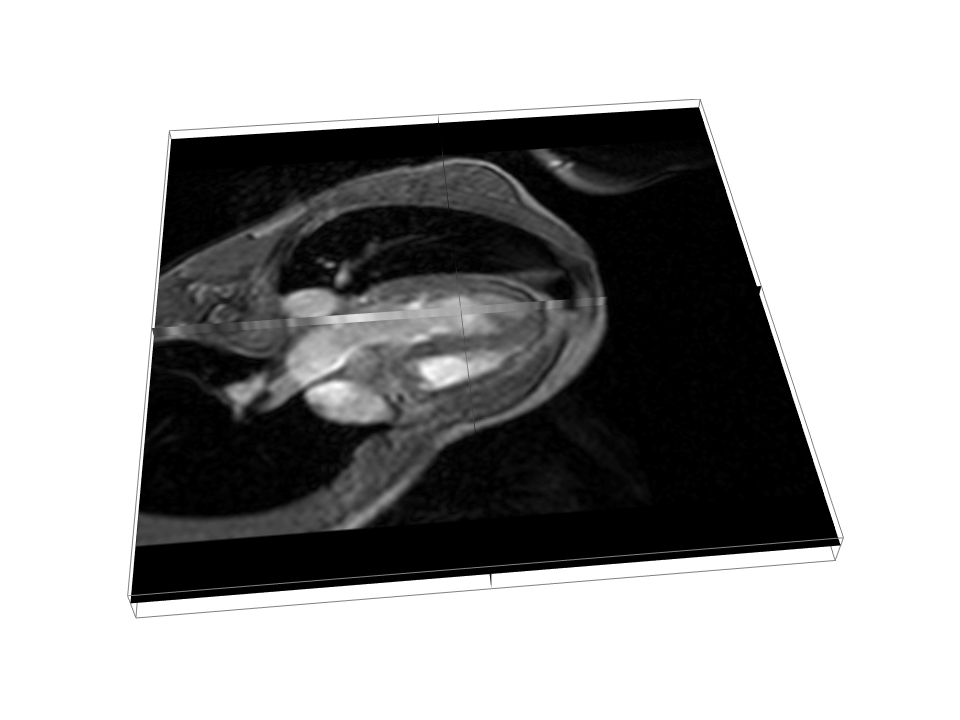
\includegraphics[width=\imglength]{images/dicom_demo}
   \caption{DICOM viewer image from \code{DicomTest}}.
   \label{fig:dicom:demo}
\end{figure}

% Previous example - was better because it was more general, but the
% site from which images were downloaded is no longer available.

%These demos automatically download sample DICOM data
%from \url{http://www.osirix-viewer.com/datasets/}.  The following
%listing provides one such example, loading an MR image of the wrist.
%Note that the image data in this example is encoded with the JPEG 2000
%format, so ImageMagick is required to decode the pixels (see
%Section \ref{sec:dicom:formats}).
%\lstset{numbers=left}
%\lstinputlisting{../../src/artisynth/demos/dicom/DicomTestImageMagic.java}
%\lstset{numbers=none}
%Lines 27--33 are responsible for downloading and extracting the sample DICOM
%zip file.  In the end, \code{dicomPath} contains a reference to the 
%desired DICOM directory on the local system.  On line 36, we create
%a regular expression pattern that will only match files ending in \texttt{.dcm}.
%On line 39, we create the viewer, which will automatically parse the 
%desired DICOM files and create a \code{DicomImage} internally.  
%We then add the viewer to the model for display purposes.  This model is
%displayed in Figure \ref{fig:dicom:wrist}.
%
%\begin{figure}[ht]
%   \centering
%   \setlengthLaTeXML{\imglength}{0.8\textwidth}{0.6\textwidth}
%   \includegraphics[width=\imglength]{images/dicom_wrist}
%   \caption{DICOM model of the wrist, downloaded from \url{http://www.osirix-viewer.com}.
%   \label{fig:dicom:wrist}}
%\end{figure}
